% presentation with pdflatex + foils package
% http://robotics.stanford.edu/~gerkey/tools/saynotopowerpoint.html

% use the foils document class, with large fonts and landscape orientation
\documentclass[20pt,landscape]{foils}

% setup the page geometry for landscape and use maximum screen real estate
\usepackage[pdftex]{geometry}
\geometry{headsep=2.0em,hscale=0.80}

% Define page margins
\setlength{\topmargin}{-1.0in}
%\addtolength{\oddsidemargin}{-0.5in}
%\addtolength{\textwidth}{1.0in}
\setlength{\oddsidemargin}{-0.5in}
\setlength{\textwidth}{10.0in}
\setlength{\textheight}{7in} 
\setlength{\foilheadskip}{-0.5in}

% title, author, date
\title{Bayes-swarm\\bayesian web spidering}
\author{Associazione BayesFor\\info@bayesfor.eu}
\date{6 ottobre 2007}

% the contents of \MyLogo are placed at the bottom center on the title slide
% and in the bottom left of other slides
\MyLogo{Associazione BayesFor, Bayes-swarm}

% basic things that we need are below
\usepackage[italian]{babel}
\usepackage[utf8]{inputenc}
\usepackage{hyperref}
\hypersetup{
  pdftitle={Bayes-swarm, bayesian web spidering and information retrieval},
  pdfauthor={Matteo Zandi, Riccardo Govoni},
  pdfsubject={Bayes-swarm, research project which aims to spider web sources and extract data with bayesian models},
  pdfpagemode={FullScreen},
  pdfborder={0 0 0}
}
\usepackage{graphicx}

% set slide command
\newcommand{\slide}[1]{\foilhead{#1}}
%\newcommand{\slide}[1]{\foilhead{#1}\noindent}

% document
\begin{document}

\LogoOff
\maketitle
\begin{center}
  
\includegraphics[width=0.3\hsize]{./figures/creative_camp_banner.png}
\end{center}

\slide{Cos'è Bayesfor?}
\LogoOn
\noindent
Una associazione che si propone di promuovere e realizzare ricerche, 
studi o sperimentazioni in materia di analisi dei dati e utilizzo di 
tecniche statistiche

\begin{center}
  http://bayesfor.eu
\end{center}

Membri:
\begin{itemize}
 	\item Bonazzi Alessandro (a.bonazzi@bayesfor.eu)
	\item Brunori Paolo (p.brunori@bayesfor.eu)
	\item Govoni Riccardo (r.govoni@bayesfor.eu)
	\item Lampronti Giulio (g.lampronti@bayesfor.eu)
	\item Zandi Matteo (m.zandi@bayesfor.eu). 
\end{itemize}

\begin{center}
http://code.google.com/p/bayes-swarm/wiki/AboutUs
\end{center}

\slide{... e Bayes-swarm?}
\noindent
E' un progetto della associazione Bayesfor, che ha l'obiettivo di fare spidering 
di fonti sul web con lo scopo di estrarre informazioni come ad esempio:
\begin{itemize}
\item Correlazione tra parole nel tempo
\item Associazioni tra parole nelle fonti
\item Correlazione tra uso di parole e notizie
\item Correlazione tra uso di parole e mercati finanziari
\end{itemize}

\begin{center}
  http://bayes-swarm.googlecode.com
\end{center}

\slide{Come funziona}
\begin{itemize}
\item Lista di fonti (siti di quotidiani italiani ed esteri, agenzie
di stampa, feed rss, etc)
\item Lista di parole "interessanti" (per ora, ma non per molto)
\item Ruby + gemme (ferret, hpricot, scrubyt, etc)
\item Mysql, database in cui sono salvate tutte le informazioni
\end{itemize}

\slide{Alcuni numeri}
\begin{itemize}
\item 7 fonti (times, guardian, euronews, ny times, al jazeera, etc)
\item 22 pagine, circa 3 per fonte (pagina principale, economica, finanziaria, etc)
\item 87 parole interessanti (china, india, bush, iraq, terror, muslim, etc)
\item circa 1000 occorrenze a settimana
\item ... attualmente a dimensioni prototipali, puo' scalare a volumi molto maggiori
\end{itemize}

\slide{Le fasi del processo di estrazione}
\begin{center}
  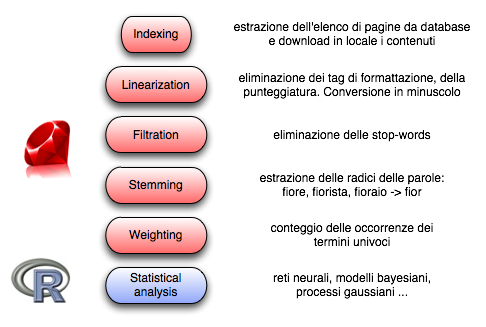
\includegraphics{./figures/elab_phases.png}
\end{center}
Il processo di estrazione utilizza un sistema modulare facilmente estendibile, 
basato sul concetto di ETL (Extact, Transform and Load) tipico dei datawarehouse.
%\begin{center}
%	http://www.miislita.com/information-retrieval-tutorial/indexing.html
%\end{center}

%\slide{Le fasi del processo di estrazione (continua)}
%\begin{center}
%	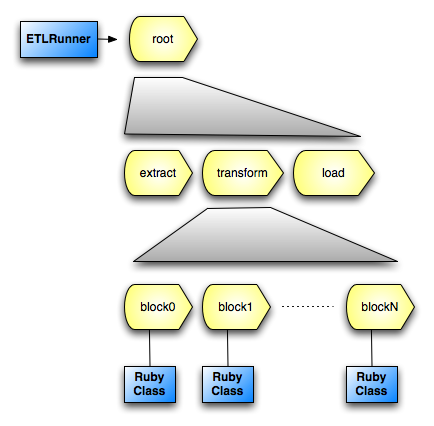
\includegraphics{./figures/etl_chains.png}
%\end{center}

\slide{Grafico serie storica bush}
\begin{center}
  \includegraphics{./figures/timeseries_bush.pdf}
\end{center}
\noindent
\begin{itemize}
\item Cosa è successo a metà agosto?
\end{itemize}

\slide{Grafici di china e india}
\begin{center}
  \includegraphics{./figures/timeseries_chinaindia.pdf}
  \includegraphics{./figures/scatterplot_chinaindia.pdf}
\end{center}
\noindent
\begin{itemize}
  \item China e india tendono ad muoversi congiuntamente?
  \item Coefficiente di correlazione $\cong 0.59$
\end{itemize}

\slide{Applicazione di modelli statistici 1/3}
\begin{center}
  \includegraphics{./figures/lm_hw_gp.pdf}
\end{center}
\noindent
\begin{itemize}
  \item Least squares: regressione semplice, presuppone una dipendenza lineare del tipo $y=a+bx$.
  \item Exponential smoothing: media di $n$ osservazioni precedenti con peso decrescente in funzione della distanza da oggi.
  \item Processo gaussiano: i parametri del modello sono funzione nel tempo.
\end{itemize}

\slide{Applicazione di modelli statistici 2/3}
\begin{center}
  \includegraphics{./figures/bi_lm_gp.pdf}
\end{center}
\noindent
Regressione semplice e processo gaussiano, caso bivariato

\slide{Applicazione di modelli statistici 3/3}
\begin{center}
  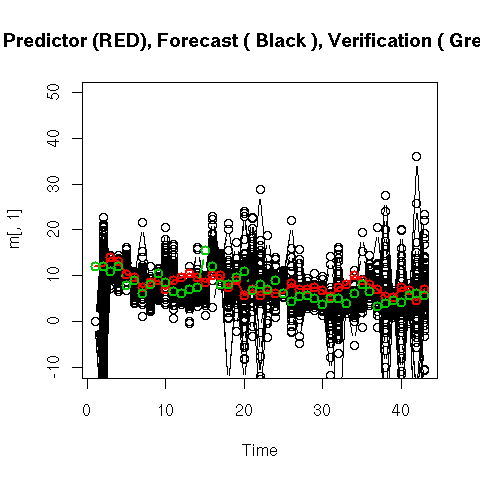
\includegraphics[width=0.4\hsize]{./figures/neural-prediction.png}
  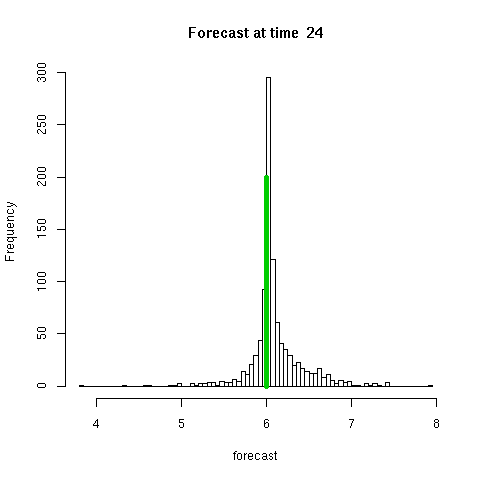
\includegraphics[width=0.4\hsize]{./figures/neural-hist.png}
\end{center}
\noindent
Neural network

\slide{Teoria dei grafi}
Utilizzo dei legami parola - pagina per creare grafi di relazioni, da cui estrarre relazioni dirette tra parole che appaiono nello stesso contesto (quando si parla di questo, si parla anche di...)
\begin{center}
  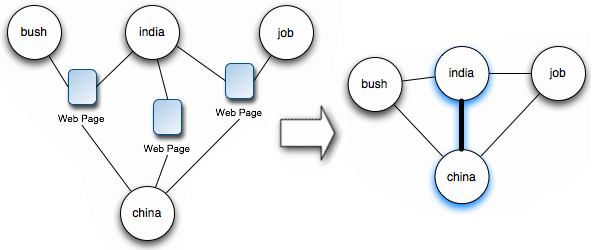
\includegraphics{./figures/graph_compression2.png}
\end{center}
\noindent
E' alla base dei sistemi di advertising piu' famosi: Amazon.com, ('chi ha comprato questo, ha comprato anche...'), Google Adwords ('se hai fatto questa ricerca, forse sei interessato anche a ...') 

\slide{Teoria dei grafi (continua)}
\begin{center}
  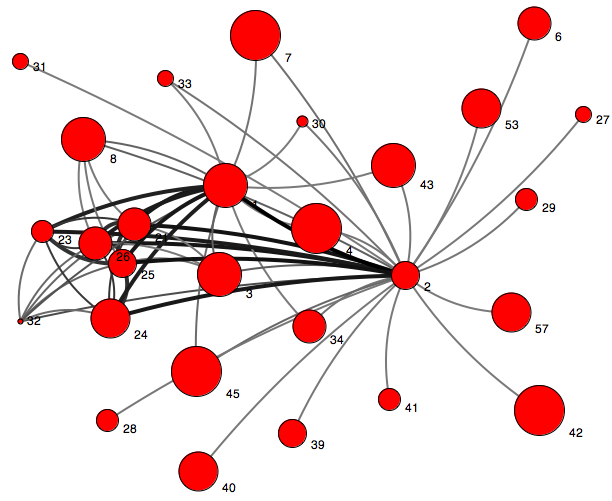
\includegraphics[width=0.4\hsize]{./figures/graphs.png}
\end{center}
\noindent
Ogni parola costituisce una 'stella', a parole con frequenza maggiore
sono associate stelle di dimensione maggiore. Ogni parola è connessa alle 
altre se sono state almeno una volta nella stessa pagina, la connessione 
è tanto più marcata quante più volte le parole si sono trovate nella stessa pagina.

\slide{Teoria dei grafi e Clustering}
\noindent
Applicare tecniche di clustering e raggruppamento (k-means, hierarchical, edge-betweenness) aiuta a identificare quali parole sono contestuali tra loro e quali invece irrilevanti. 

\begin{center}
  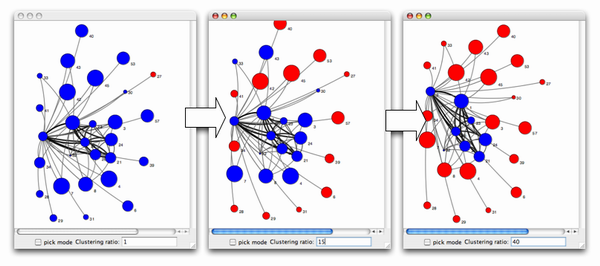
\includegraphics{./figures/graph_clustering.png}
\end{center}

\slide{Da qui in avanti}
\begin{itemize}
	\item aumento del corpus di dati oggetto di analisi
	\item analisi sulle forme di distribuzione dell'informazione derivanti dal web 2.0: i feed rss
	\item sperimentazione di altre tecniche statistiche (SVD, ...)
	\item sperimentazione su corpus di dati preesistenti di grandi dimensioni (il dataset Enron)
\end{itemize}

\slide{Grazie per l'attenzione}
\noindent
\begin{center}
  http://bayesfor.eu\\http://bayes-swarm.googlecode.com
  
  \huge{domande?}
\end{center}

\end{document}
